% A planar lattice: a long, skew basis and a reduced one (generated by a script).
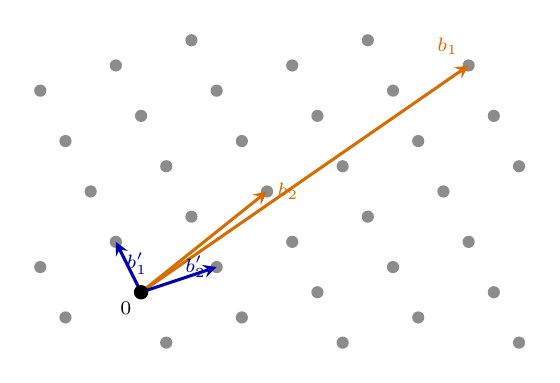
\begin{tikzpicture}[x=0.32cm,y=0.32cm]
\clip (-4.5,-2.5) rectangle (15.5,10.5);
\fill[black!45] (15,-2) circle (2.2pt);
\fill[black!45] (8,-2) circle (2.2pt);
\fill[black!45] (11,-1) circle (2.2pt);
\fill[black!45] (14,0) circle (2.2pt);
\fill[black!45] (1,-2) circle (2.2pt);
\fill[black!45] (4,-1) circle (2.2pt);
\fill[black!45] (7,0) circle (2.2pt);
\fill[black!45] (10,1) circle (2.2pt);
\fill[black!45] (13,2) circle (2.2pt);
\fill[black!45] (-3,-1) circle (2.2pt);
\fill[black!45] (0,0) circle (2.2pt);
\fill[black!45] (3,1) circle (2.2pt);
\fill[black!45] (6,2) circle (2.2pt);
\fill[black!45] (9,3) circle (2.2pt);
\fill[black!45] (12,4) circle (2.2pt);
\fill[black!45] (15,5) circle (2.2pt);
\fill[black!45] (-4,1) circle (2.2pt);
\fill[black!45] (-1,2) circle (2.2pt);
\fill[black!45] (2,3) circle (2.2pt);
\fill[black!45] (5,4) circle (2.2pt);
\fill[black!45] (8,5) circle (2.2pt);
\fill[black!45] (11,6) circle (2.2pt);
\fill[black!45] (14,7) circle (2.2pt);
\fill[black!45] (-2,4) circle (2.2pt);
\fill[black!45] (1,5) circle (2.2pt);
\fill[black!45] (4,6) circle (2.2pt);
\fill[black!45] (7,7) circle (2.2pt);
\fill[black!45] (10,8) circle (2.2pt);
\fill[black!45] (13,9) circle (2.2pt);
\fill[black!45] (-3,6) circle (2.2pt);
\fill[black!45] (0,7) circle (2.2pt);
\fill[black!45] (3,8) circle (2.2pt);
\fill[black!45] (6,9) circle (2.2pt);
\fill[black!45] (9,10) circle (2.2pt);
\fill[black!45] (-4,8) circle (2.2pt);
\fill[black!45] (-1,9) circle (2.2pt);
\fill[black!45] (2,10) circle (2.2pt);
\draw[->,>=stealth,orange!85!black,line width=1.1pt] (0,0)--(13,9) node[above left,font=\scriptsize]{$b_1$};
\draw[->,>=stealth,orange!85!black,line width=1.1pt] (0,0)--(5,4) node[right,font=\scriptsize]{$b_2$};
\draw[->,>=stealth,blue!70!black,line width=1.1pt] (0,0)--(-1,2) node[below right,font=\scriptsize]{$b_1'$};
\draw[->,>=stealth,blue!70!black,line width=1.1pt] (0,0)--(3,1) node[left,font=\scriptsize]{$b_2'$};
\fill[black] (0,0) circle (2.6pt) node[below left,font=\scriptsize]{$0$};
\end{tikzpicture}
